%!TEX root = ../main.tex
%TODO: Redo the flowchart with updated and more specific steps

The input to our problem is a fiducial marker $F$ to provide the object position in the real world; and a 3D mesh $M$ which will be rendered in Augmented Reality. The method will calculate the properties of a set of light sources $L_i$, specifically position, rotation, intensity and color. In order to analyze the luminance ($L()$), a $360^{\circ}$ panoramic image is required, generated as a pre-processing step as explained in chapter \ref{theory}. The entirety of the process is depicted in the flowchart in Figure \ref{flowch}, and each step is consequently described in more detail.

\begin{figure}[H] 
  \centering
  \setlength{\unitlength}{\textwidth} 
    \begin{picture}(1,0.5)
       \put(-0.1,0){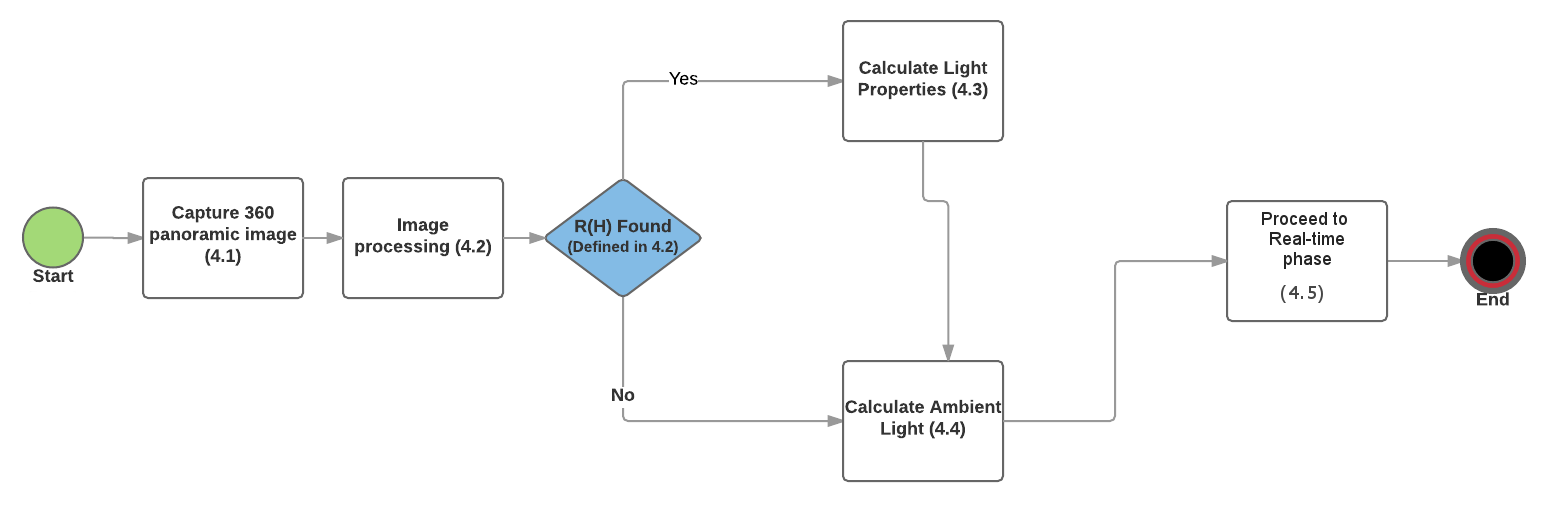
\includegraphics[width=1.3\unitlength]{Figures/Flowchart.png}}
       
    \end{picture}
    \caption{Our method in a nutshell.}
    \label{flowch}
\end{figure} 

\section{Capture $360^{\circ}$ panoramic image}
In this work panoramic images are used as a pre-process and therefore it's not within the scope of the method to define a new way of capturing $360^{\circ}$ images. The application we used to procure a spherical panoramic image within the device itself is Google Street View.
The origin of the virtual world for placing and orienting the mesh $M$ within this reference is asked to the user by rotating the virtual reflective sphere so that the view of the room aligns with that of the section of the real room that the camera is facing. This will also simplify calculations of light orientations later on.

\section{Light source filtering}
Once the panoramic image is loaded and oriented the first step is to reduce the chromatic representation into luminance. This is achieved with the following equation:

\begin{equation}
  \forall \  P_{ij}; \quad L(R_{ij},G_{ij},B_{ij}) = 0,2126 \cdot R_{ij} + 0,7152 \cdot G_{ij} + 0,0722 \cdot B_{ij} 
\end{equation}

Where $L$ is the luminance obtained at D65 white point and $P$ is the pixel in the $i,j$ position of the image \newline
The contrast ratio has to be adjusted, so that the regions with high luminance are more clearly separated. 

\begin{equation}
     g(i,j) = \alpha \cdot L(i,j) + \beta
\end{equation}

Where $g(i,j)$ is the adjusted image, $L(i,j)$ is the original grayscale image and $\alpha$ and $\beta$ are the brightness and contrast constants respectively, determined by parameter tuning. We carried out the parameter tuning in a trial-and-error basis, propose initial extreme values and run the program, changing the values in order to achieve the best result. The values that worked in the implementation were $\alpha = 220$ and $\beta = 255$.
In order to prevent outlier pixels and noise from causing false positives, we normalize $g(i,j)$ as follows:

\begin{equation}
    L(P_{ij}) = \frac{ 2 \cdot P_{ij} }{min(L) + max(L)},
\end{equation}

Where $min(L)$ and $max(L)$ are the overall minimum and maximum luminance values in the image. 
\newline
The result of these steps is a black and white image with the rough shape of the light source, we call these shapes \emph{regions of high luminance}. If there are no regions of high luminance in the image whatsoever it means that no relevant light sources were found. A region of high luminance in the image is formally defined as follows:

\begin{equation}
    R(H) = \{p_{00}, p_{01}, ... , p_{mn}\},
\end{equation}
 where $p_{ij}$ is the pixel in the i,j position of the image, so that 
\[
    L(p_{ij}) > 0.9 \cdot max(L(p_{ij})) 
\]

The region must also be side-wise connected, so the pixels must be adjacent.\newline
Regions of high luminance are for the most part characterized by much noise and artifacts, caused by clear objects, reflections of light sources on highly reflective surfaces, and even light sources that are so far away in the distance, but don't really contribute an important amount of light to the area of interest. Therefore, it's necessary to also add further filtering to the pipeline. \newline
The amount of light that a lighting source contributes to a given scene is directly proportional to the emission area of that source. When analyzing a photograph this area translates to the pixel size of the light source in the image. So we consider this to be a good measure for filtering. Figuring what constitutes an acceptable region size to determine if we have to filter a the light source is a challenging problem. The approach we took to face this problem is to define a percentage of the width and height of the overall image as a threshold in search for the best solution. The size filter is then:

\begin{equation}
    width(R(H)) \cdot height(R(H)) \geq k \cdot W \cdot H
\end{equation}

Where $k$ is the threshold, in the implementation the value that yielded the best results was $k = 0.004$; $W$ and $H$ are the total image width and height.\newline

Even after all the filtering we capped the maximum amount of light to 8 in practice, due to performance concerns.\newline

\section{Calculate light properties}
We need to calculate position, orientation, intensity, and color for each light, remembering that we have the original full color image available. We note that it is not trivial to calculate the position from just a single point of view as input. Even though the simulation would be a lot more robust if the actual position with respect to the camera was simulated, there is just not enough information to calculate it in this method. For that reason all the lights are placed at the best approximation we could calculate with the data we have, even knowing it's not very accurate. \newline
With this in mind, all the other properties can be calculated.

\begin{enumerate}
\item  \textbf{Orientation}: The pixel coordinates (x,y) of the centroid of each light within the luminance panorama are saved. The image is projected on a sphere. The camera casts rays onto the sphere from 4 different points of view, 0\degree , 90\degree, 180\degree  and 270\degree. If the ray hits a white pixel and the pixel coordinates of the hit are approximately those of the centroid the light direction is calculated as follows:
\begin{equation}
    O(L_p) = -2 \cdot (N_h \cdot C_r) N_h + C_r
\end{equation}
Where $O(L_p)$ is the orientation of the pth light source, $N_h$ is the sphere normal on the hit point, $C_r$ and is the camera ray direction.\newline
This process is depicted in Figure \ref{camMov} for further clarification. The figure shows the vectors, the camera orbiting the reflective sphere and the four distinct points of view with which the camera reconstructs the entire $360^{\circ}$ environment.
\begin{figure}[H] 
  \centering
  \setlength{\unitlength}{\textwidth} 
    \begin{picture}(0.75,0.5)
       \put(-0.1,0){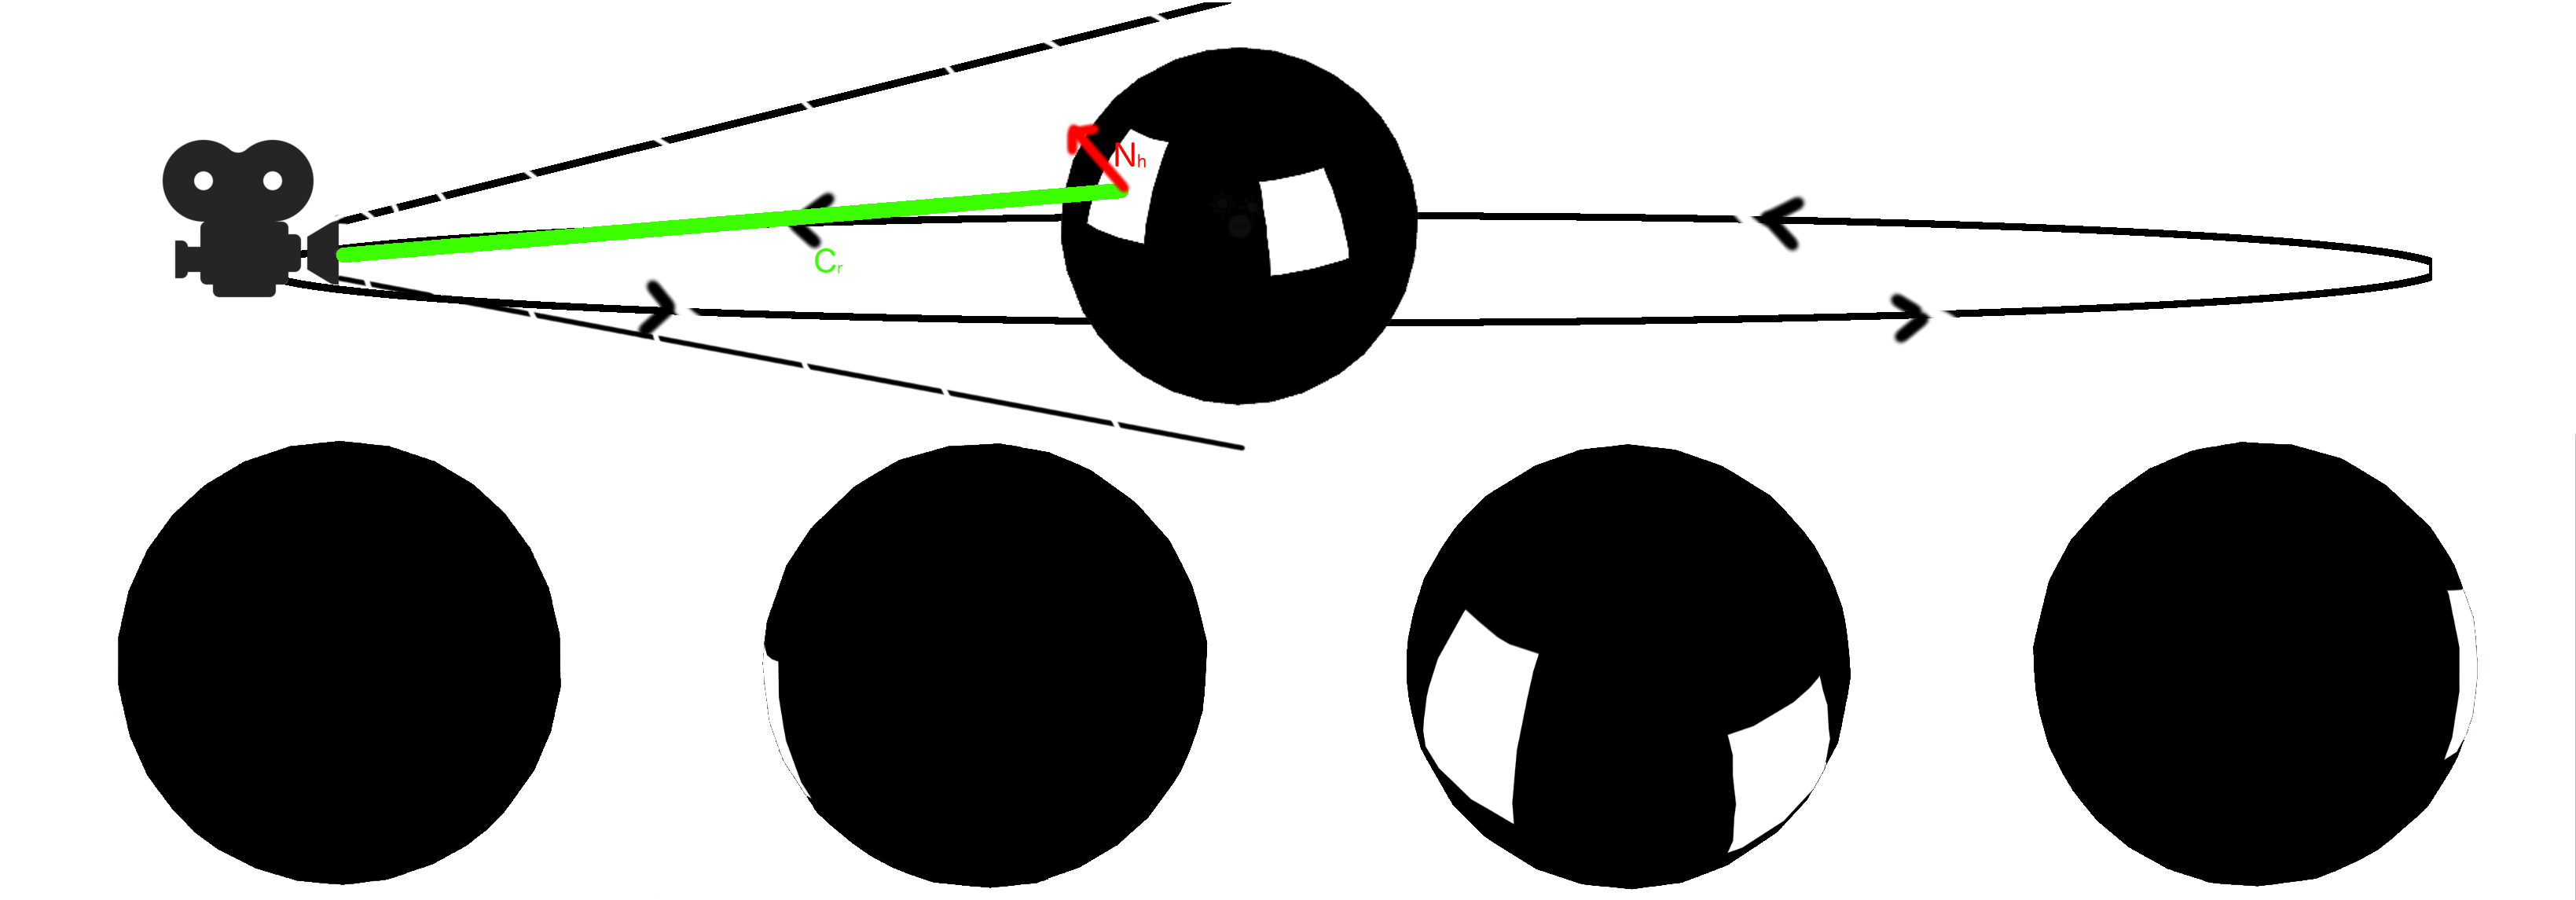
\includegraphics[width=1.0\unitlength]{Figures/camMov.png}}
       
    \end{picture}
    \caption{Illustration of how the light orientations are calculated based on the virtual reflective sphere.}
    \label{camMov}
\end{figure} 

\item \textbf{Position}:We normalize the orientation vector calculated before and take those x, y and z components as the unit position vector. We subsequently approximate the distance using triangle similarity and the device's known camera parameters and a known object size. We use the average of a light source's height to approximate the desired distance:
\begin{equation}
   D = \frac{f \cdot h(O_r) \cdot h(L)}{h(O_p) \cdot h(s)},
\end{equation}

where $f$ is the camera aperture size, $h(O_r)$ and $h(O_p)$ are the real object height in millimeters and the image object height in pixels respectively; $h(L)$ is the height of the full image and $h(s)$ is the camera sensor height.

\item \textbf{Color}: Storing both versions of the panorama, one in full color and another one after processing, allows us to have both the color and the luminance information. Once a light source is detected, the equivalent area in the color image is averaged to determine the color of the light source.
\item \textbf{Intensity}: There are two factors that influence the intensity of a light as perceived by a camera, the light size and the color temperature. The light's color temperature in Kelvin is calculated using the approximation proposed by \cite{mccamy1992}, as follows:
\begin{equation}
    T(C_p) = -949.86315 + 6253.80338 ^ {\frac{-n}{0.92159} } + 28.70599 ^{\frac{-n}{0.20039} } + 0.00004 ^ {\frac{-n}{0.07125} }
\end{equation}
\begin{equation}
n = {\frac{0.23881\cdot R + 0.25449\cdot G - 0.58291\cdot B}{0.11109\cdot R - 0.85406\cdot G + 0.52289\cdot B} }
\end{equation}

Where $R, G, B$ are the red, green and blue components of the light color.\newline 
The size analogy is given by the integral of the region of high luminance with respect to the full image. The light intensity is finally expressed by:
\begin{equation}
I(L_p) = T(C_p) \cdot \int_R L(i) \,dx
\end{equation}
Where $L(i)$ is the output image of the luminance analysis and $R$ is the $p^{th}$ region of high luminance.\newline 

\end{enumerate}

\section{Calculate ambient light}
Environment mapping is an image-based technique to approximate the appearance of the overall light conditions of an environment. This is accomplished by means of a precomputed texture image mapped as a far-away environment surrounding. Said surrounding is usually a geometric surface, when \cite{Blinn76} first introduced the method they used a sphere. Nowadays there are other alternatives, such as cube, paraboloid, pyramid or cylinder maps. The principle for each surface is the same, but the way to map a planar image onto the surface varies per surface.\newline
Since a panoramic image of the environment is already available using it to implement environment mapping would be an adequate use of resources. In order to generate an environment map it is necessary that the panorama is made into a High Dynamic Range image. This is because the Low Dynamic Range image captured directly from the device camera fails to capture the information necessary to simulate correct color balance, shadows, and highlights of the lighting environment; ultimately producing both inaccurate and less visually pleasing results. This has been illustrated by \cite{DebevecRSO}.\newline 
A relatively easy and effective way to make an image into an HDR version is a technique called Tone Mapping, in which versions with different exposure values of the same image are blended together to include the full range of highlights and shadows of the overexposed and underexposed versions in a single image. Since asking the user to capture the environment more than once would have a bad impact on user friendliness, and also it's highly unlikely that the produced image would have the exact same framing every time, the different exposure values for the Tone Mapping will be produced altering the brightness and contrast values of the base image using equation 4.2 once again. After that the HDR image is produced using the \cite{Debevec} weighting algorithm.\newline
It's important to disclaim that the Tone Mapping process will not yield an actual HDR image. In the first place, it will be a standard 24 bit image in the $0...255$ range, with highlight and shadow valued clipped. The upside to still going through this process nonetheless is that the environment will be described in a richer way, capturing the bright areas and the shadows better than the standard exposure image.

\section{Real-time Phase}
The original sphere panoramic photograph is widely used in the real time phase. It is used to create a cubemap of the real environment to be used as ambient lighting, to calculate the ambient contribution of the diffuse shaders and to fake reflections for the specular shaders.
\begin{enumerate}

\item Cubemap: The image coordinates are first converted to polar and divided into four regions by latitude $-\Pi/4 < \theta < \Pi/4 , \Pi/4 < \theta < 3\Pi/4, 3\Pi/4 < \theta < 5\Pi/4, 5\Pi/4 < \theta < 7\Pi/4$. These represent either one of the four faces of the cube, top or bottom. The projected coordinate is given by:
\begin{equation}
P = (1, tan(\phi), \frac{cot(\theta)}{cos(\phi)})
\end{equation}
 The projected point is always on the top if $ \frac{cot(\theta)} { (1/\sqrt{2}) }> 1$ or $tan(\theta)< \frac{1}{\sqrt{2}}$ \newline
 
 The projected points for each face of the cube are composed into an image and each image stitched together to create a cross cube map.
 
 \item Ambient contribution: The environment lighting contribution is done via shader. The ambient contribution is reduced to a single value in the range of $0$ and $1$ and then the albedo color component of the object's shader is multiplied by this value. The result is a dimmer color when the ambient light is low. 
 The ambient contribution value itself is obtained by calculating the mean of the luminance panoramic image, since this already contains the lighting information of the room and the different intensities and distributions.
 
 \item Reflections: Another way the panoramic image is used to enhance the realism of the composted scene is by generating accurate reflections of the real scene. The cubemap from a previous step is also used to fake reflections. A vector is cast from every vertex of the object along its normal and intersected with the cubemap generated from the panoramic image. The color is mixed with the albedo according to the specularity defined for the material to simulate reflection, this information is calculated in advance and used at runtime. This works well enough because we know beforehand that the scene is static, there will only be one non-animated object throughout the full execution.
 
 \item Shadows: During early experiments it became clear that one of the bigger differences between real and virtual object were a product of the shadows as well as the light. There are two main problems when it comes to casting shadows for virtual objects in AR, one is the fact that there has to be an object underneath the 3D model to cast the shadow on, but this object has to be as unobtrusive as possible. If the goal is to achieve realism having the object appearing on a pedestal for the sake of casting shadows is counter productive. This issue is worked around by using a transparent material that receives shadows. The other main problem is that the shadows of real objects are deformed when cast on other objects, this problem is beyond the scope of this method, as it would require the program to have a notion of the geometry of the real space.\newline
 The shadows work quite well, but are not as soft as real shadows. A masking scheme using a gradient texture was tried to make softer shadows but it didn't work, because the color was contaminated and it made apparent that there was a shadow catching plane. 
 
\end{enumerate}